\section{Context Compression}
\label{sec:context.compression}

\subsection{Motivation}

In a long-horizon agent rollout, the working context contains the original
instructions, model-generated actions, and environment observations.  If every
turn is appended, the context eventually reaches the model's context limit.
Even before that point, a very long context increases rollout cost and can
degrade instruction following.  Merely applying a summarizer at inference time
does not address the training problem: after old interactions are removed, the
summary determines which information is available to every subsequent action.
Summary generation is therefore part of the policy, rather than a lossless
preprocessing operation.

\subsection{Compaction Mechanism}

Both SUPO~\citep{lu2025scaling} and
CompactionRL~\citep{li2026compactionrl} make this idea trainable.  Let the
interaction history after turn $t$ be
\begin{align}
    h_t=(p_0,z_1,\ldots,z_t),
    \qquad z_i=(\ambf_i,o_i),
    \label{eq:compaction.history}
\end{align}
where $p_0$ is the fixed initial context, $\ambf_i$ is a policy-generated
assistant action span, and $o_i$ is the corresponding environment observation.
When a deterministic length threshold is reached, a fixed summarization
instruction $q_{\mathrm{sum}}$ is appended and the same trainable policy
generates
\begin{align}
    S_t\sim\pi_\theta(\cdot\mid h_t\oplus q_{\mathrm{sum}}).
    \label{eq:compaction.summary}
\end{align}
The rollout then resumes from a reconstructed context of the generic form
\begin{align}
    \bar h_t
    =
    p_{\mathrm{keep}}
    \oplus u_{\mathrm{resume}}(S_t)
    \oplus \operatorname{Tail}_\kappa(z_1,\ldots,z_t).
    \label{eq:compaction.reconstruction}
\end{align}
Here $\operatorname{Tail}_\kappa(z_1,\ldots,z_t)
=(z_{t-\kappa+1},\ldots,z_t)$ denotes the $\kappa$ most recent complete
action--observation pairs.  SUPO uses $\kappa=0$, while CompactionRL uses
$\kappa=2$ by default and reduces it when necessary to fit the context budget.  The retained
prefix $p_{\mathrm{keep}}$ is also implementation-specific.  These details do
not change the shared causal mechanism: the generated summary replaces most of
the old history and affects the terminal task reward through all future
decisions.

\begin{figure}[H]
    \centering
    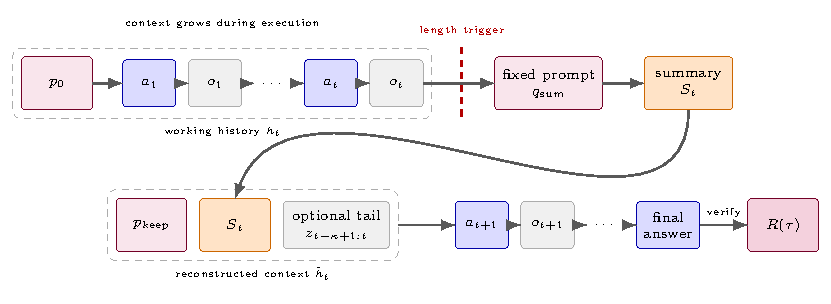
\includegraphics[width=0.98\linewidth]{figures/context_compaction_mechanism.pdf}
    \caption{Shared trainable compaction mechanism in SUPO and CompactionRL.
    A deterministic length rule triggers a fixed summary instruction, and the
    same policy that performs task actions generates the summary.  The working
    context is reconstructed from retained initial context, the summary, and an
    optional recent-history tail before the same rollout continues.  The final
    task reward trains both execution and summary tokens.  The exact retained
    prefix and history tail are method-specific.}
    \label{fig:context.compaction.mechanism}
\end{figure}

It is useful to make precise what is learned.  In both methods, the
\emph{time of compaction is forced by a length rule}; the policy does not learn
whether or when to compact.  The policy learns the summary tokens and the
ordinary execution tokens.  Partition a compacted rollout into context-bounded
multi-turn segments $\tau=(\sigma_1,\ldots,\sigma_K)$.  A typical nonfinal
segment has the form
\begin{align}
    \sigma_k
    =
    \big(
        p_{\mathrm{keep}},
        u_{\mathrm{resume}}(S_{k-1}),
        \operatorname{Tail}_{\kappa_k},
        (\ambf_{k,1},o_{k,1}),\ldots,
        (\ambf_{k,m_k},o_{k,m_k}),
        q_{\mathrm{sum}},S_k
    \big),
    \label{eq:compaction.segment}
\end{align}
where $\ambf_{k,t}$ is an assistant action span and $o_{k,t}$ is its
environment observation.  The previous summary is absent from $\sigma_1$; the
final segment omits $q_{\mathrm{sum}},S_K$ and instead ends with the final
answer.

Each assistant action span is itself a token sequence; for example,
$\ambf_{k,t}=(y_{k,t,1},\ldots,y_{k,t,L_{k,t}})$, and the summary $S_k$
also contains many policy-generated tokens.  Flatten the generated tokens in
the execution and summary spans of $\sigma_k$ in chronological order as
$y_{k,1},\ldots,y_{k,n_k}$.  Let $x_{k,i}$ be the complete visible prefix
immediately before token $y_{k,i}$ is sampled.  Thus observations are
incorporated into later prefixes $x_{k,i}$ but are not themselves optimized
tokens.  Let $\Mcal(\tau)$ collect all such policy-token coordinates $(k,i)$.
Figure~\ref{fig:compacted.rollout.indexing} visualizes this multi-turn
structure.

\begin{figure}[H]
    \centering
    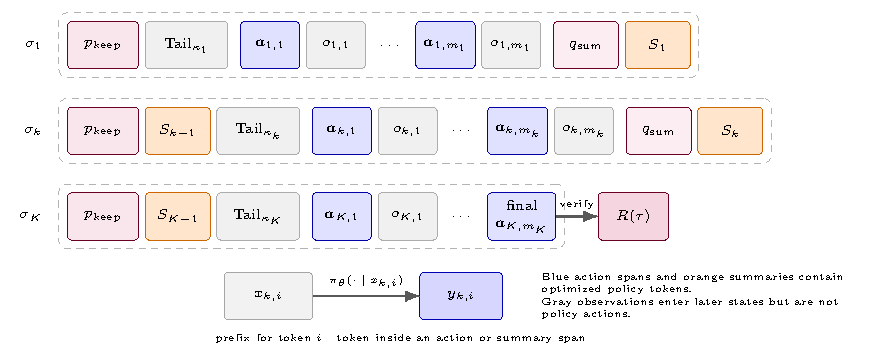
\includegraphics[width=0.98\linewidth]{figures/compacted_rollout_indexing.pdf}
    \caption{Multi-turn segment structure and policy-token indexing.  Every
    segment begins with retained context, the preceding summary when available,
    and an optional recent tail, followed by assistant action--observation
    pairs.  A nonfinal segment ends by generating its next summary.  After
    flattening only the policy-generated execution and summary tokens, $(k,i)$
    selects token $y_{k,i}$ and $x_{k,i}$ is its pre-token prefix.
    Observation tokens affect later prefixes but do not belong to
    $\Mcal(\tau)$.}
    \label{fig:compacted.rollout.indexing}
\end{figure}

With this indexing, the score-function identity gives
\begin{align}
    \grad_\theta \Jcal(\theta)
    =
    \Embb_{\tau\sim\pi_\theta}
    \left[
        R(\tau)
        \sum_{(k,i)\in\Mcal(\tau)}
        \grad_\theta\log\pi_\theta(y_{k,i}\mid x_{k,i})
    \right].
    \label{eq:compaction.policy.gradient}
\end{align}
Thus a separate summary-quality reward is not required: a summary is reinforced
when the information it preserves helps the later policy obtain a larger task
reward.  The main difference between the two algorithms is how the common
terminal reward is converted into an advantage for each token.

\subsection{CompactionRL: PPO with Cross-Segment GAE}

CompactionRL uses a fixed context budget $C$ and triggers compaction when
\begin{align}
    C-\lvert h_t\rvert<T_{\mathrm{comp}}.
\end{align}
It treats each $(\ambf_i,o_i)$ pair as atomic, so a tool call is not separated
from its observation.  After sampling $S_t$, the new context contains the
system prompt, a fixed resume template carrying $S_t$, and the $\kappa$ most
recent action--observation pairs.  The default is $\kappa=2$, reduced if needed
to fit the context budget.  We use the context-bounded segments
$\sigma_1,\ldots,\sigma_K$ defined in
Equation~\eqref{eq:compaction.segment}; execution and summary tokens in every
segment are optimized under the same rollout reward.  Here $\Mcal$ denotes all
token coordinates $(k,i)$ in these segments.

\paragraph{Token-normalized PPO objective.}
For generated token $y_{k,i}$ in $\sigma_k$, conditioned on its visible prefix
$x_{k,i}$, define the ratio against the rollout policy by
\begin{align}
    \rho_{k,i}(\theta)
    :=
    \frac{\pi_\theta(y_{k,i}\mid x_{k,i})}
         {\pi_{\theta_{\mathrm{old}}}(y_{k,i}\mid x_{k,i})}.
\end{align}
CompactionRL maximizes
\begin{align}
    \Jcal_{\mathrm{CompactionRL}}(\theta)
    :=
    \frac{1}{\lvert\Mcal\rvert}
    \sum_{(k,i)\in\Mcal}
    \min\left\{
        \rho_{k,i}(\theta)\widehat A_{k,i},
        \operatorname{clip}\left(
            \rho_{k,i}(\theta),1-\epsilon,1+\epsilon
        \right)\widehat A_{k,i}
    \right\}.
    \label{eq:compactionrl.objective}
\end{align}
The single denominator counts all optimized tokens in the batch.  This avoids
giving every compacted segment equal weight regardless of its length, which
would over-weight rollouts split into many short segments.  It does not make
all rollouts equally weighted: a rollout containing more optimized tokens can
still contribute more terms.

\paragraph{Cross-segment generalized advantage estimation.}
Let segment $\sigma_k$ contain $n_k$ optimized tokens.  CompactionRL first
computes a local GAE
\begin{align}
    \delta_{k,i}
    &:=
    r_{k,i}
    +\gamma V_\phi(x_{k,i+1})
    -V_\phi(x_{k,i}), \\
    A_{k,i}^{\mathrm{loc}}
    &:=
    \sum_{\ell=0}^{n_k-i}
    (\gamma\lambda)^\ell\delta_{k,i+\ell}.
    \label{eq:compactionrl.local.gae}
\end{align}
If this calculation is performed independently on every segment, placing the
shared terminal reward at every segment boundary would make that reward appear
too close to tokens in early segments.  Let
\begin{align}
    N_{>k}:=\sum_{m>k}n_m
\end{align}
be the number of optimized tokens in later segments of the same rollout.
CompactionRL corrects the local estimate by
\begin{align}
    \widehat A_{k,i}
    :=
    (\gamma\lambda)^{N_{>k}}A_{k,i}^{\mathrm{loc}}.
    \label{eq:compactionrl.cross.gae}
\end{align}
In particular, the terminal-reward contribution at token $(k,i)$ is
discounted by
$(\gamma\lambda)^{N_{>k}+n_k-i}$, matching its token distance to the final
outcome in the concatenated rollout.  This exact-distance statement concerns
the terminal-reward term: Equation~\eqref{eq:compactionrl.cross.gae} rescales
the entire local advantage, including its value residuals, so it is an
approximation rather than ordinary GAE over one uninterrupted state sequence.
The paper also does not fully specify the token-level placement of
$r_{k,i}$ or whether the value-regression target uses the local or corrected
advantage.

A critic $V_\phi$ is trained with the standard PPO value-regression loss, so
the method can estimate token-dependent advantages even with one rollout per
prompt.  In the reported implementation, the critic is pretrained and receives
two updates per policy update.  It uses
\begin{align}
    \lambda=1-\frac{1}{\alpha l},
    \qquad \alpha=1.5,
\end{align}
where the paper calls $l$ the response length but does not specify its exact
interpretation across multi-response execution segments.

\subsection{SUPO: GRPO with Rollout-Level Group Advantages}

SUPO augments a multi-turn tool-use MDP with a length threshold $L$.  Once the
threshold is crossed, the policy is prompted to summarize the current
subtrajectory.  The next subtrajectory starts from the original prompt plus
that summary; unlike CompactionRL, no recent action--observation tail is kept.
The practical rollout algorithm also discards the action--observation pair
that caused the threshold crossing before requesting the summary.  This keeps
the summary itself within the training context limit; the paper's theoretical
transition, in contrast, retains that pair.  A complete rollout
$\tau^j$ with $I^j$ summaries is consequently stored as $I^j+1$
subtrajectories.

\paragraph{Advantage estimation before splitting.}
For each prompt, SUPO samples $G$ complete compacted rollouts from
$\pi_{\theta_{\mathrm{old}}}$ and obtains terminal rewards
$\{R^1,\ldots,R^G\}$.  Its GRPO-style advantage is computed over these
original rollouts:
\begin{align}
    \widehat A^j
    :=
    \frac{
        R^j-\operatorname{mean}(\{R^{j'}\}_{j'=1}^{G})
    }{
        \operatorname{std}(\{R^{j'}\}_{j'=1}^{G})
    }.
    \label{eq:supo.advantage}
\end{align}
The same scalar $\widehat A^j$ is then assigned to every execution and summary
token in all $I^j+1$ subtrajectories originating from rollout $j$.  The
important detail is that $R^j$ appears only once in the group statistics.
Computing the mean and standard deviation after splitting would repeat $R^j$
$I^j+1$ times and bias the baseline toward rollouts that compact more often.
As with ordinary GRPO, the implementation must handle a group whose rewards
have zero standard deviation, but the paper does not state the safeguard used.

\paragraph{SUPO objective and overlong mask.}
Write response span $\ambf_t^j$ as
$\ambf_t^j=(y_{t,1}^j,\ldots,y_{t,L_t^j}^j)$, and let
$x_{t,\ell}^j$ be the visible prefix before token $y_{t,\ell}^j$.  The
token-level ratio is
\begin{align}
    \rho_{t,\ell}^j(\theta)
    :=
    \frac{
        \pi_\theta(y_{t,\ell}^j\mid x_{t,\ell}^j)
    }{
        \pi_{\theta_{\mathrm{old}}}
        (y_{t,\ell}^j\mid x_{t,\ell}^j)
    }.
\end{align}
Let $\Mcal^j$ contain all generated-token positions in all subtrajectories of
rollout $j$, and let
\begin{align}
    m^j
    :=
    \Imbb\left\{
        \tau^j \text{ emits a final answer before truncation by } H
        \text{ or } S
    \right\}.
\end{align}
Here $H$ and $S$ are the maximum numbers of interaction steps and
summaries.  Crucially, $m^j$ is a \emph{completion mask}, not a success mask:
a completed but incorrect answer still has $m^j=1$ and therefore remains a
negative training example.  An overlong rollout instead ends because an
external compute limit is reached, without producing a final answer.  Its
failure reward does not reveal which earlier decision caused nontermination.
Because SUPO broadcasts the same $\widehat A^j$ to every execution and summary
token, retaining a negative objective term for such a rollout would suppress
all of those decisions together, including summaries that may have supported
useful continued search.  This creates a shortcut incentive to avoid
summarization and force an early answer.

\begin{figure}[H]
    \centering
    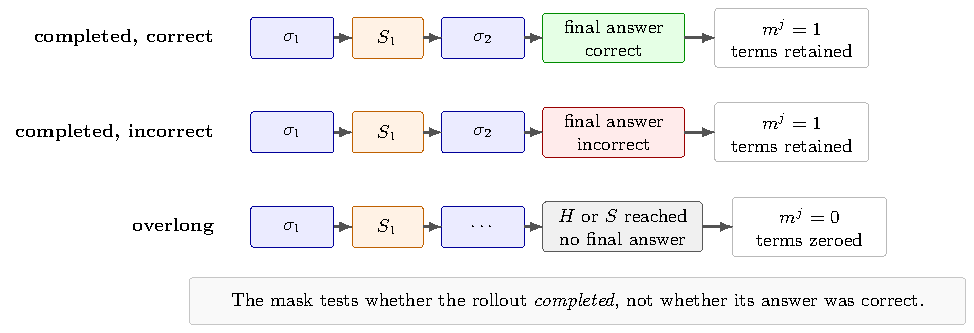
\includegraphics[width=0.98\linewidth]{figures/supo_overlong_mask.pdf}
    \caption{Effect of SUPO's overlong mask.  Both correct and incorrect
    completed rollouts contribute policy-gradient terms.  Only a rollout
    truncated by the step limit $H$ or summary limit $S$ before emitting a
    final answer has all of its token-level terms zeroed.}
    \label{fig:supo.overlong.mask}
\end{figure}

SUPO then maximizes the globally token-normalized objective
\begin{align}
    \Jcal_{\mathrm{SUPO}}(\theta)
    :=
    \frac{1}{\sum_{j=1}^{G}\lvert\Mcal^j\rvert}
    \sum_{j=1}^{G}
    \sum_{(t,\ell)\in\Mcal^j}
    m^j
    \min\left\{
        \rho_{t,\ell}^j(\theta)\widehat A^j,
        \operatorname{clip}\left(
            \rho_{t,\ell}^j(\theta),
            1-\epsilon_{\mathrm{low}},
            1+\epsilon_{\mathrm{high}}
        \right)\widehat A^j
    \right\}.
    \label{eq:supo.objective}
\end{align}
The mask removes the overlong rollout's own policy-gradient terms.  As written,
its reward can still affect the detached group mean and standard deviation in
Equation~\eqref{eq:supo.advantage}.  In the paper's ablation, removing the mask
causes summarization usage to collapse and reduces conditional success.  The
reported experiments use $G=8$, asymmetric clipping
$\epsilon_{\mathrm{low}}=0.20$ and
$\epsilon_{\mathrm{high}}=0.28$, and no KL or entropy penalty.

\paragraph{Comparison.}
The apparent tension between the papers is resolved by the unit at which the
advantage is computed.  CompactionRL avoids group-relative estimation and uses
a critic to give each token a temporally corrected advantage; it therefore
supports group size one.  SUPO remains critic-free by computing one relative
advantage per \emph{complete rollout before segmentation} and broadcasting it
to all of that rollout's tokens.  SUPO thereby handles the variable number of
subtrajectories without duplicating rewards in the group baseline, but it
cannot distinguish an early summary token from a late execution token within
the same rollout.  The compaction mechanism is shared; the principal
algorithmic difference is fine-grained temporal credit assignment versus a
coarser, critic-free group-relative baseline.